\documentclass[12pt,a4paper]{article}
\usepackage[UTF8]{ctex}
\usepackage{amsmath,amssymb}
\usepackage{xcolor}
\usepackage{hyperref}
\usepackage{geometry}
\usepackage{graphicx}
\geometry{margin=2.5cm}

\title{QAOA Traveling Salesman / QAOA 旅行商问题}
\author{QuoNic}
\date{}

\begin{document}
\maketitle

\begin{center}
\textbf{Algorithms / 算法} | 难度：高级 | 预计时间：25 分钟
\end{center}

\tableofcontents
\newpage

\section{为什么需要？}

QAOA 旅行商问题是 QAOA 在组合优化中的经典应用。

\subsection{经典局限}
\begin{itemize}
  \item 旅行商问题是 NP-hard 问题
  \item 经典算法需要指数时间
  \item 对于大规模问题，经典方法效率低
\end{itemize}

\subsection{量子优势}
\begin{itemize}
  \item QAOA 可以提供比经典近似算法更好的解
  \item 对噪声有鲁棒性
  \item 理论上可以达到最优解
\end{itemize}

\subsection{实际应用}
\begin{itemize}
  \item 物流配送
  \item 电路设计
  \item 基因组测序
\end{itemize}

\section{快速上手}

\begin{verbatim}
from quonic.algorithms import qaoa_tsp

# 旅行商问题
cities = [(0,0), (1,0), (1,1), (0,1)]
result = qaoa_tsp(cities, p=2)
print(f'Shortest distance: {result.distance}')
print(f'Route: {result.route}')
\end{verbatim}

\textbf{预期输出}：
\begin{verbatim}
Shortest distance: 4.0
Route: [0, 1, 2, 3]
\end{verbatim}

\section{原理详解}

\subsection{电路图}

\begin{center}
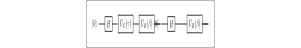
\includegraphics[width=0.6\textwidth]{../../images/qaoa_tsp_circuit.svg}
\end{center}

\subsection{数学推导}

旅行商问题的目标函数：
\begin{equation}
\min \sum_{i,j} d_{ij} x_{ij} \quad \text{s.t.} \quad \sum_j x_{ij} = 1, \sum_i x_{ij} = 1
\end{equation}

QAOA 编码：
\begin{equation}
C(x) = \sum_{i,j} d_{ij} x_{ij} + \lambda \sum_i (1 - \sum_j x_{ij})^2
\end{equation}

\subsection{几何解释}

QAOA 旅行商问题在参数空间中寻找最短路径。量子计算机负责制备态和测量，经典优化器负责更新参数。

\section{代码详解}

\begin{verbatim}
from quonic.algorithms import qaoa_tsp

# qaoa_tsp(cities, p, optimizer)
# cities: 城市坐标列表
# p: QAOA 层数
# optimizer: 优化器

result = qaoa_tsp(
    cities=[(0,0), (1,0), (1,1), (0,1)],
    p=2,
    optimizer='cobyla'
)

# result.distance: 最短距离
# result.route: 最优路径
# result.params: 优化后的参数
print(f'Shortest distance: {result.distance}')
print(f'Route: {result.route}')
\end{verbatim}

\section{进阶用法}

\subsection{场景 1：不同层数}

\begin{verbatim}
from quonic.algorithms import qaoa_tsp

cities = [(0,0), (1,0), (1,1), (0,1)]

for p in [1, 2, 4]:
    result = qaoa_tsp(cities, p=p)
    print(f'p={p}: Distance={result.distance}')
\end{verbatim}

\subsection{场景 2：不同城市数}

\begin{verbatim}
from quonic.algorithms import qaoa_tsp
import numpy as np

# 不同城市数
for n in [4, 6, 8]:
    cities = [(np.random.rand(), np.random.rand()) for _ in range(n)]
    result = qaoa_tsp(cities, p=2)
    print(f'n={n}: Distance={result.distance}')
\end{verbatim}

\subsection{场景 3：实际物流问题}

\begin{verbatim}
from quonic.algorithms import qaoa_tsp

# 实际物流问题
cities = [
    (0, 0),    # 仓库
    (1, 2),    # 客户 1
    (3, 1),    # 客户 2
    (2, 4),    # 客户 3
    (4, 3),    # 客户 4
]

result = qaoa_tsp(cities, p=3)
print(f'Optimal route: {result.route}')
print(f'Total distance: {result.distance}')
\end{verbatim}

\section{适用场景}

\subsection{物流配送}

QAOA 旅行商问题可以用于物流配送路线规划。例如，快递员需要访问多个客户，找到最短路径可以节省时间和成本。

\subsection{电路设计}

QAOA 旅行商问题可以用于电路设计中的布线优化。例如，在芯片设计中，找到最短的连线路径可以减少延迟和功耗。

\section{常见问题}

\subsection{QAOA 旅行商问题和经典旅行商问题有什么区别？}

QAOA 旅行商问题使用量子策略，可以利用量子叠加探索更大的解空间。

\subsection{QAOA 旅行商问题的精度如何？}

精度取决于层数和参数优化策略。

\section{学习路径}

\subsection{前置知识}
\begin{itemize}
  \item QAOA
  \item 旅行商问题
  \item 组合优化
\end{itemize}

\subsection{继续学习}
\begin{itemize}
  \item QAOA MaxCut
  \item QAOA 背包问题
  \item 量子优化
\end{itemize}

\section{完整示例代码}

\subsection{示例 1：基本 QAOA 旅行商问题}

\begin{verbatim}
from quonic.algorithms import qaoa_tsp

cities = [(0,0), (1,0), (1,1), (0,1)]
result = qaoa_tsp(cities, p=2)
print(f'Shortest distance: {result.distance}')
\end{verbatim}

\section{下载}

\begin{itemize}
  \item [qaoa\_tsp.py](https://github.com/ChrisLee0721/QuoNic/blob/main/examples/qaoa_tsp/qaoa_tsp.py)
\end{itemize}

\end{document}
